\chapter{Conclusion}
\label{ch:conclusion}

This chapter covers the final state of the NIPEN project.
It at also discusses the state of all the requirements of the project.
At the end it talks about what the customer should do about future work on this project.

\lhead{Chapter 16. \emph{Conclusion}} 

\section{Fulfillment of requirements}

This section discusses how our project fulfills the requirements of the project. 
It explains the state of all the requirements and if they were completed. Each requirement had a priority which halped us identify what was important for us to focus on.

\subsection{Fulfillment of functional requirements}

This subsection describes the functional requirements for the product and their state after the project completion.
Our initial requirements were that this platform should both recive and deliver health data. 
The requirements were revised during the project with feedback from the customer.
The customer felt it was sufficent that the integration platform was able to receive health data and that it was more important to have a good sync with Microsoft HealtVault. 
The final product can out receive and deliver health data but there is no authentication on the delivering part in this prototype. 

\textbf{Fulfillment of functional requirements for the integration platform}

\begin{table}[H]
\begin{center}
\begin{tabular}{ | c | p{9cm} | c | c | }
  \hline
  ID & Description & Priority & State\\
  \hline\noalign{\smallskip}\noalign{\smallskip}\hline
  FIP1	& The IP shall support REST endpoints for receiving heart rate data models expressed as JSON strings   & High & Completed\\
  FIP2	& The IP shall support REST endpoints for receiving weight data models expressed as JSON strings       & High & Completed \\
  FIP3	& The IP shall support REST endpoints for forwarding heart rate models (using JSON) to other systems.  & High & Completed \\
  FPI4	& The IP shall support REST endpoints for forwarding weight models (using JSON).                       & High & Completed \\
  \hline
\end{tabular}
\end{center}
\caption{Fulfillment of functional requirements for Integration platform}
\label{table:fulfillemntofrequirements}
\end{table}

\subsection{Fulfillment of the functional requirements for the web front-end}

This subsection describes the functional requirements for the web front-end and its state after the project completion. 
In figure \ref{figure:front-endfinal} the design and final version can be seen. 
The most import job of the web front-end was to display the data in an informative way.
We landed on using grafs to display the data. 
We also tried to make it look like the clients page by using their color scheme.

\begin{figure}[H]
\centering
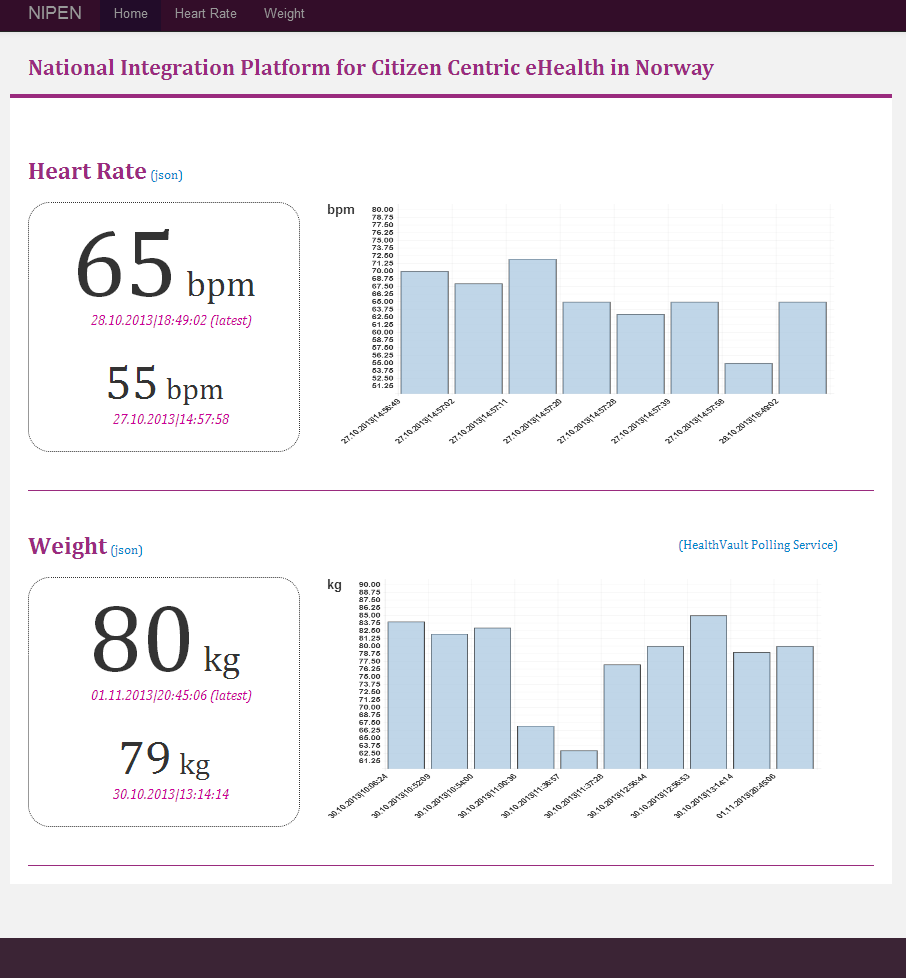
\includegraphics[scale=0.50]{../Figures/front-endfinal.png}
\caption{Front-end final}
\label{figure:front-endfinal}
\end{figure}

\textbf{Functional requirements for the web front-end}

\begin{table}[H]
\begin{center}
\begin{tabular}{ | c | p{9cm} | c | c |}
  \hline
  ID & Description & Priority & Status\\
  \hline\noalign{\smallskip}\noalign{\smallskip}\hline
  FW1	& The web frontend shall display the data stored by the Integration Platform using charts.	& High & Completed \\
  FW2	& The web frontend shall use Helsenorge color palette                                       & Low & Completed \\
  \hline
\end{tabular}
\end{center}
\caption{Fulfillment of functional requirements for the web front-end}
\label{table:fulfillemntofwebfront-end}
\end{table}

\subsection{Fulfillment of functional requirements for the heart rate application}

This subsection describes the functional requirements for the heart rate application and its state after the project completion.
In figure \ref{figure:appfinal} the design and final version can be seen.
The app is very simple but functional. 
The goal of the app was to be able to, with the help of the camera, to capture the heart rate of people.
Then with the click of a button transmitt the data to NIPEN.


\begin{figure}[H]
\centering

\includegraphics[scale=0.20]{../Figures/appfinal.png}
\caption{Heart rate application final}
\label{figure:appfinal}
\end{figure}

\textbf{Fulfillment of functional requirements for Heart rate application}

\begin{table}[H]
\begin{center}
\begin{tabular}{ | c | p{9cm} | c | c |}
  \hline
  ID & Description & Priority & Status\\
  \hline\noalign{\smallskip}\noalign{\smallskip}\hline
  FHR1	& The application shall measure user’s heart rate using the device camera    & High & Completed \\
  FHR2	& The application shall display the last measurement on the screen.          & Med & Completed \\
  FHR3	& The application shall forward the data to the IP using its REST endpoint.  & High & Completed \\
  \hline
\end{tabular}
\end{center}
\caption{Fulfillment of functional requirements for the heart rate application}
\label{table:fulfillemntofapp}
\end{table}

\subsection{Fulfillment of functional requirements for Weight application}

This subsection describes the functional requirements for the weight application and its state after the project completion.
In figure \ref{figure:weightapp} the design and final version can be seen.
The goal of this app was to get weight data from Microsoft HealthVault and send it to NIPEN.

\begin{figure}[H]
\centering

\includegraphics[scale=0.20]{../Figures/weightappfinal.png}
\caption{Fulfillment of weight application}
\label{figure:weightappfinal}
\end{figure}

\textbf{Functional requirements for Weight application}

\begin{table}[H]
\begin{center}
\begin{tabular}{ | c | p{9cm} | c | c |}
  \hline
  ID & Description & Priority & Status\\
  \hline\noalign{\smallskip}\noalign{\smallskip}\hline
  FHV1	& The application shall fetch weight data from HealthVault.						      & High & Unkown \\
  FHV2	& The application shall show the user the data it has fetched.              & Med & Unkown \\
  FHV3	& The application shall forward the data to the IP using its REST endpoint. & High & Unkown \\
  \hline
\end{tabular}
\end{center}
\caption{Fulfillemnt of functional requirements for Weight application}
\label{table:fulfillemntweightapp}
\end{table}

\subsection{Fulfillment of non-funcional requirements}
This subsection describes the non-functional requirements and its state after the project completion. 

\begin{table}[H]
\begin{center}
\begin{tabular}{ | c | c |p{6.5cm} | c | c |}
  \hline
  ID & Category & Description & Priority & Status\\
  \hline\noalign{\smallskip}\noalign{\smallskip}\hline
  NF1 & Documentation & The system shall be thoroughly documented, both at the code level and by the document ‘project report’.
  & High & Completed \\
  NF2 & Documentation & Although security and privacy are not requirements for the product they are important topics to be discussed in the documentation.
  & High & Completed \\
  NF3 & Open-source	& The product shall be released under a permissive license approved by the product owner.
  & High & Completed \\
  NF4 & Interoperability & The system shall provide a good degree of interoperability. Third party application developers should be put in the condition to develop third party (interoperable) solutions rapidly.
  & High & Completed \\
  NF5 & Interoperability & A number of two-three prototype applications shall be developed in order to showcase the functionality of the system.
  & High & Completed \\
  NF6 & Accessibility & The web-frontend should have a good degree of accessibility. It should have a rather simple design and use a user-provided palette.
  & Low & Completed \\
  \hline
\end{tabular}
\end{center}
\caption{Fulfillment of non-functional requirements}
\label{table:fullfilmentnonfunctionalreq}
\end{table} 

\section{Further work}

Our NIPEN implementation and the belonging applications are mostly a proof of concept. 
The most important task of the client to do next will be to figure out if there is an interest in Helsenorge for this type of system.
The most important factor for this system is the value it delivers to the educated medical professionals. 
If this is something that gives the medical professionals additional value and makes it easier for them to understand the patiens health. 
A cost and benefit analysis of this system needs to be done to analyse the total value this system will give will be an important factor in deciding where to go next. 
The thought is that citizens can collect all types of health data and that even though their measurements might be imprecise that quantity of health data will overall improve the quality. 
This system is definitely possible to implement at a larger scale at a high cost.
The toughest part will be to convince the medical professionals to start using new methods and systems. 
Many will be pessimistic for this kind of system knowing that the data at some degree could not be dependent upon.
The important part to consider then is that even though specific data might be inaccurate it will be a lot easier to analyse trends and get a sense of the citizens habits. 

The value of this system can be hard to measure but already many people today do these kinds of measurements and the adaption is increasing. 
Earlier this year Pew Research Center’s Internet \& American Life Project released their findings of the role of Internet and technology in health and wellness. 
Their report, Tracking for Health can be found here http://pewinternet.org/Reports/2013/Tracking-for-Health.aspx, is focused on how people self-track.
In the research paper they found that 7 out of 10 adults track their health.
While 1 in 5 use technology to log this. 
What is important to note from the findings they did is that over half of those who keep a record of their health indicate that their tracking and recordkeeping has changed their approach to health.
The conclusion that can be taken from this is that the act of tracking alone affects the overall health and mindset of the citizen. 

\subsection{Third-party applications}

We developed three applications all interacting with our implementation of NIPEN. 
The idea behind making a portal like this is to open the API up to all developers so the NIP can be interoperable between all platforms, systems, applications and users. 
The ideal goal is to have a platform that reaches all types of users. 
The total cost of the project can be lowered by this because support for the system can be done by the developers of the different third-party applications. 
It is also possible for some developers to develop proxies for popular third-party applications.


\section{Summary}
In this chapter we have looked at what requirements our project have fulfilled. 
We have also discuessed what the next steps for pursuing the continues development of this platform. 

We are glad that we manage to implement most of the requirements meaning we made a realistic assumptions of what we could accomplish in the given time with the members we had. 
Although some of the syncronisation did not work ideeal it was not cause by our system but by third-party systems not working ideally. 
This project is an interesting idea and finding a way to unify the collection of health data of citizens will lead to a better understanding of citizen health and an easier overview of what can be improved for a better quality of life. 